\documentclass[12pt,a4paper]{article}
\usepackage[margin=2cm]{geometry}
\usepackage{xeCJK}
\usepackage{fontspec}
\setCJKmainfont{Noto Serif CJK TC}[Script=CJK]
\usepackage{amsmath,amssymb}
\usepackage{graphicx}
\usepackage{fancyhdr}
\setlength{\headheight}{14.5pt}
\addtolength{\topmargin}{-2.5pt}
\usepackage{hyperref}
\usepackage{listings}
\usepackage{enumitem}
\usepackage{titlesec}
\usepackage{caption}
\usepackage{indentfirst}
\usepackage{float}
\usepackage{forest}
\setlength{\parindent}{2em}
\pagestyle{fancy}
\fancyhf{}
\cfoot{\thepage}
\linespread{1.3}

\usepackage{multirow}
\usepackage{booktabs}   % 放在 preamble
\usepackage{graphicx}
\usepackage{afterpage}

% tikz tools for ER diagram
\usepackage{tikz}
\usetikzlibrary{shapes,positioning,calc}
\colorlet{lightgray}{gray!20}


\usepackage{minted}
\setminted{
    linenos,                % 行號
    frame=lines,            % 上下框線
    framesep=5pt,           % 程式碼與邊框距離
    numbersep=8pt,          % 行號與程式碼距離
    fontsize=\scriptsize,   % 字體大小
    breaklines,             % 自動換行
    tabsize=4,              % tab 寬度
    rulecolor=\color{black},% 框線顏色
    xleftmargin=1.5em       % 左側縮排
}


\title{資料庫管理 HW03}
\author{B12508026戴偉璿}
\date{}

\begin{document}

\maketitle

\lhead{資料庫管理 HW03}
\rhead{B12508026戴偉璿}

\begin{enumerate}
    \item 
    \begin{enumerate}
        \item Left join all advisors(e) and their advisees(s), if someone has no advisee, then s would be NULL.
        \begin{minted}{sql}
select e.id, e.name from employee as e
left join employee s on e.id=s.supervisor_id
where s.supervisor_id is null;
        \end{minted}
        \item Find the latest store id of each employee before 2025-01-05 and left join to the employee table.
        \begin{minted}{sql}
select e.id as employee_id, h.store_id
from employee e
left join employee_store_history h
on e.id = h.employee_id
and h.start_date_time=(
    select max(h2.start_date_time)
    from employee_store_history h2
    where h2.employee_id = e.id
        and h2.start_date_time <= '2025-01-05'
    );           
        \end{minted}
        \item Using \texttt{limit 1} to obtain the first store id and \texttt{limit 1 offset 1} to obtain the second store id (after skipping the first one), then join them to produce the final result.
        \begin{minted}{sql}
select e.id as employee_id,
    (select h1.store_id from employee_store_history h1 where h1.employee_id=e.id order by h1.start_date_time limit 1) as first_store_id,
    (select h2.store_id from employee_store_history h2 where h2.employee_id=e.id order by h2.start_date_time limit 1 offset 1) as second_store_id
from employee e;
        \end{minted}
        \item Calculating the total quantity purchased for each product, then ordering by total quantity and product\_id, using \texttt{limit 2 offset 3} to find the 4th and 5th products. Finally, joining with purchase\_detail and purchase tables to get the required information.
        \begin{minted}{sql}
with total_qty as(
    select pd.product_id as product_id, sum(pd.qty) as total_qty, count(*) as purchase_count
    from purchase_detail pd
    group by pd.product_id
),
target_product as(
    select product_id
    from total_qty
    order by total_qty desc, product_id asc
    limit 2 offset 3
)
select p.id as product_id, p.name as product_name, pu.store_id as store_id, count(*) as purchase_count, sum(pd.qty) as total_qty
from target_product tp
join product p on tp.product_id = p.id
join purchase_detail pd on pd.product_id = p.id
join purchase pu on pd.purchase_no = pu.purchase_no
group by p.id, p.name, pu.store_id
order by p.id, pu.store_id;
        \end{minted}
        \item First choose the target product ids by ranking the total purchased quantity, then cross join with store table to get all combinations of target products and stores. Finally, left join with purchase and purchase\_detail tables to get the required information.
        \begin{minted}{sql}
with total_qty as(
    select pd.product_id as product_id, row_number() over(order by sum(pd.qty) desc, pd.product_id asc) as rnk
    from purchase_detail pd
    group by pd.product_id
),
target as(
    select product_id
    from total_qty 
    where rnk >= 4 and rnk <= 5
)
select t.product_id as id, p.name as name, s.id as store_id, coalesce(sum(pd.qty), 0) as amount, coalesce(count(distinct pu.purchase_no), 0) as cnt
from target t --target store id
cross join store s
left join purchase pu on pu.store_id = s.id
left join purchase_detail pd on pu.purchase_no = pd.purchase_no and t.product_id = pd.product_id
join product p on p.id = t.product_id 
group by s.id, t.product_id, p.name
order by t.product_id, s.id;          
        \end{minted}
        \item Calculate the total spending of each member in each store, then rank them within each store based on the total spending. Using \texttt{rank()} instead of \texttt{row\_number()} to handle ties in spending amounts. While ranking, using \texttt{partition by} to separate rankings for each store. 
        \begin{minted}{sql}
select sa.store_id as store_id, sa.member_id as member_id, sum(sd.unit_price*sd.qty) as amount, rank() over(partition by sa.store_id order by sum(sd.unit_price*sd.qty) desc) as rnk

from sales sa
join sales_detail sd on sd.receipt_no = sa.receipt_no
where member_id is not null
group by sa.store_id, sa.member_id
order by sa.store_id, rnk;
        \end{minted}
    \end{enumerate}
    \item
    \begin{enumerate}
        \item First, I identified the hard questions based on the number of total answers and correct answers. Then, for each hard question, I found each user’s first correct submission and ranked the users by cost time and submission timestamp. Finally, I counted the number of hard questions where each user ranked in the top 3 and kept only those who appeared in at least two questions.\\
        Fig.~\ref{fig:2a} shows the leaderboard of top users appearing in at least two hard questions.
        \begin{figure}[H]
            \centering
            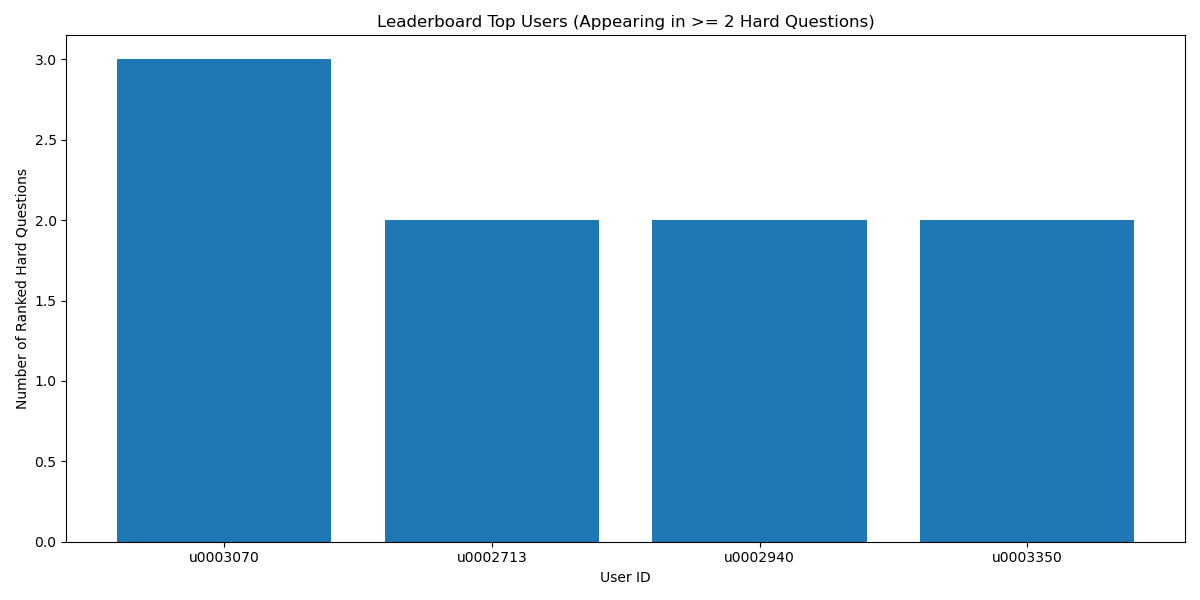
\includegraphics[width=0.8\textwidth]{code/2a_leaderboard.png}
            \caption{Leaderboard of Top Users Appearing in at Least Two Hard Questions}
            \label{fig:2a}
        \end{figure}
        Following is my source code, I used DuckDB to execute the SQL query and Matplotlib to visualize the results.
        \begin{minted}{python}
import duckdb
import matplotlib.pyplot as plt

con = duckdb.connect('my_database.db')

df = con.sql("""
-- list the hard questions
with hard_questions as(
    select question_id as id, count(*) as total_ans, sum(is_correct) as total_ac
    from answers
    group by question_id
    having total_ans >= 1000 and total_ac <= 500
),-- list the rank for all users
first_correct_pre as(
    select question_id, user_id, cost_time, created_at, rank() over(partition by question_id, user_id order by created_at asc) as rnk
    from answers
    where is_correct = 1
),-- first correct for each user
first_correct as(
    select question_id, user_id, cost_time, created_at
    from first_correct_pre
    where rnk = 1
),--rank users for hard questions
usr_rnk as(
    select question_id, user_id, rank() over(partition by question_id order by cost_time asc, created_at asc) as rnk
    from first_correct fc
    join hard_questions hq on hq.id = fc.question_id
)
select user_id, count(distinct question_id) as appr_cnt
from usr_rnk
where rnk <= 3
group by user_id
having appr_cnt >= 2
order by appr_cnt desc, user_id asc;
""").df()
print(df)

plt.figure(figsize=(12,6))
plt.bar(df["user_id"].astype(str), df["appr_cnt"])
plt.xlabel("User ID")
plt.ylabel("Number of Ranked Hard Questions")
plt.title("Leaderboard Top Users (Appearing in >= 2 Hard Questions)")
plt.tight_layout()
plt.savefig("2a_leaderboard.png")
plt.show()            
        \end{minted}
        \item Using the same CTEs as in 2a to find the users who ranked in the top 3 for hard questions. Then I calculated their scores based on the given scoring system. Finally, I kept only those users with a total score of at least 5.\\
        Fig.~\ref{fig:2b} shows the leaderboard of top users with a score of at least 5.
        \begin{figure}[H]
            \centering
            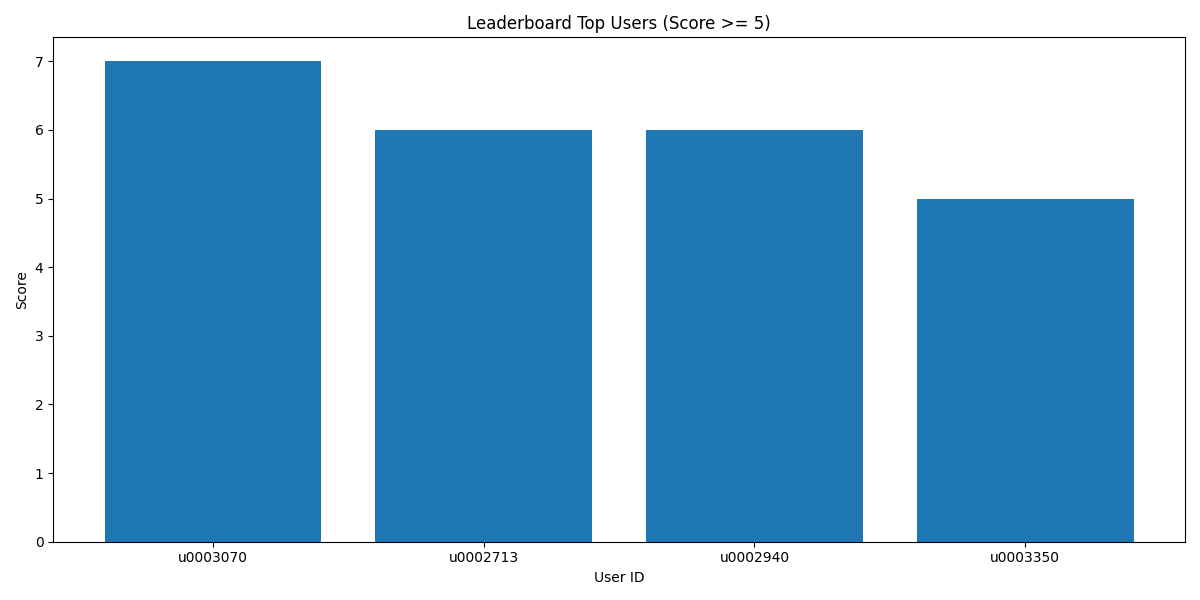
\includegraphics[width=0.8\textwidth]{code/2b_leaderboard.png}
            \caption{Leaderboard of Top Users with a Score of at Least 5}
            \label{fig:2b}
        \end{figure}
        Following is my source code:
        \begin{minted}{python}
import duckdb
import matplotlib.pyplot as plt

con = duckdb.connect('my_database.db')

df = con.sql("""
-- list the hard questions
with hard_questions as(
    select question_id as id, count(*) as total_ans, sum(is_correct) as total_ac
    from answers
    group by question_id
    having total_ans >= 1000 and total_ac <= 500
),-- list the rank for all users
first_correct_pre as(
    select question_id, user_id, cost_time, created_at, rank() over(partition by question_id, user_id order by created_at asc) as rnk
    from answers
    where is_correct = 1
),-- first correct for each user
first_correct as(
    select question_id, user_id, cost_time, created_at
    from first_correct_pre
    where rnk = 1
),--rank users for hard questions
usr_rnk as(
    select question_id, user_id, rank() over(partition by question_id order by cost_time asc, created_at asc) as rnk
    from first_correct fc
    join hard_questions hq on hq.id = fc.question_id
)
select user_id, 
       sum(
           cast(rnk = 1 as int) * 5 +
           cast(rnk = 2 as int) * 2 +
           cast(rnk = 3 as int) * 1
       ) as score
from usr_rnk
where rnk <= 3
group by user_id
having score >= 5
order by score desc, user_id asc;
""").df()
print(df)

plt.figure(figsize=(12,6))
plt.bar(df["user_id"].astype(str), df["score"])
plt.xlabel("User ID")
plt.ylabel("Score")
plt.title("Leaderboard Top Users (Score >= 5)")
plt.tight_layout()
plt.savefig("2b_leaderboard.png")
plt.show()            
        \end{minted}
    \end{enumerate}
\end{enumerate}

\end{document}